\documentclass[12pt]{article}
\usepackage{amscd,amssymb,amsmath,latexsym,enumerate}
\usepackage{tikz}
\usepackage{tikz-cd}
\usetikzlibrary{calc}
\usepackage{xcolor}

\newcommand{\tick}[1]{\filldraw[black!100,line width=0.5mm,fill=none]{#1} ellipse (0.0 and 0.2)}

\begin{document}

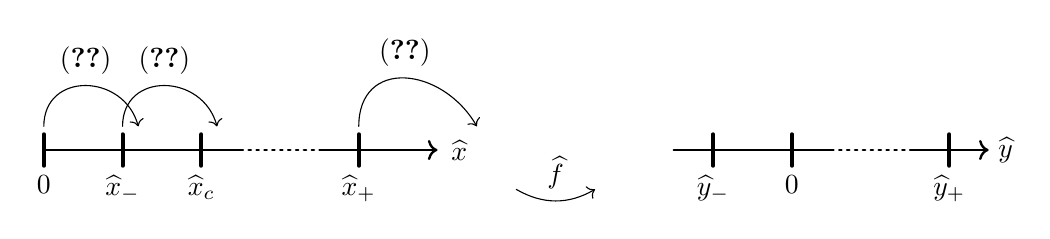
\begin{tikzpicture}[line join = round, line cap = round]
		\coordinate (a) at (0.0,0.3);
		\coordinate (b) at (0.0,-0.2);
		\coordinate (bb) at (0.0,-0.8);
		\coordinate (r) at (0.2,0.0);
		\coordinate (l0) at (-6.5,0);
		\tick{(l0)};
		\coordinate (l0a) at ($(l0) + (a)$);
		\coordinate[label=below:{$0$}] (l0b) at ($(l0) + (b)$);
		\coordinate (l1) at (-5.5,0);
		\tick{(l1)};
		\coordinate (l1a) at ($(l1) + (a)$);
		\coordinate (l1ar) at ($(l1) + (a) + (r)$);
		\draw[->] (l0a) to[out=90, in=105, looseness=1.5] node[midway,above,inner sep=4pt] {\eqref{stat:slower-start}} (l1ar);
		\coordinate[label=below:{$\widehat{x}_-$}] (l1b) at ($(l1) + (b)$);
		\coordinate (l2) at (-4.5,0);
		\tick{(l2)};
		\coordinate (l2ar) at ($(l2) + (a) + (r)$);
		\draw[->] (l1a) to[out=90, in=105, looseness=1.5] node[midway,above,inner sep=4pt] {\eqref{stat:slower-between}} (l2ar);
		\coordinate[label=below:{$\widehat{x}_c$}] (l2b) at ($(l2) + (b)$);
		\coordinate (l3) at (-4,0);
		\coordinate (l4) at (-3,0);
		\coordinate (l5) at (-2.5,0);
		\tick{(l5)};
		\coordinate (l5a) at ($(l5) + (a)$);
		\coordinate[label=below:{$\widehat{x}_+$}] (l5b) at ($(l5) + (b)$);
		\coordinate (lr) at (-1.5,0);
		\coordinate[label=left:{$\widehat{x}$}] (lrr) at (-1,0);
		\coordinate (lrra) at ($(lrr) + (a)$);
		\draw[->] (l5a) to[out=90, in=120, looseness=1.5] node[midway,above,inner sep=4pt] {\eqref{stat:slower-end}} (lrra);
		\draw [-,color=black,line width=0.3mm] (l0)--(l3);
		\draw [-,color=black,dotted,line width=0.3mm] (l3)--(l4);
		\draw [->,color=black,line width=0.3mm] (l4) -- (lr);
		\coordinate (ml) at (-0.5,-0.5);
		\coordinate (mr) at (0.5,-0.5);
		\draw[->] (ml) to[bend right] node[midway,above,inner sep=4pt] {$\widehat{f}$} (mr);
		\coordinate (rl) at (1.5,0);
		\coordinate (r1) at (2,0);
		\tick{(r1)};
		\coordinate[label=below:{$\widehat{y}_-$}] (r1b) at ($(r1) + (b)$);
		\coordinate (r2) at (3,0);
		\tick{(r2)};
		\coordinate[label=below:{$0$}] (r2b) at ($(r2) + (b)$);
		\coordinate (r3) at (3.5,0);
		\coordinate (r4) at (4.5,0);
		\coordinate (r5) at (5,0);
		\tick{(r5)};
		\coordinate[label=below:{$\widehat{y}_+$}] (r5b) at ($(r5) + (b)$);
		\coordinate[label=right:{$\widehat{y}$}] (rr) at (5.5,0);
		\draw [-,color=black,line width=0.3mm] (rl)--(r3);
		\draw [-,color=black,dotted,line width=0.3mm] (r3)--(r4);
		\draw [->,color=black,line width=0.3mm] (r4) -- (rr);
		\end{tikzpicture}

\end{document}